\documentclass[12pt,letterpaper]{article}

\usepackage{graphicx}
\usepackage[top=1in, bottom=1in, right=1in, left=1in]{geometry}

\renewcommand*\rmdefault{ppl}

\def\WorkTitle{The Title}
\def\WorkAuthor{The Author}
\def\WorkType{novel}
\def\PrintRoyalties{25\%}
\def\DigitalRoyalties{50\%}
\def\PaymentMechanism{PayPal} % Or check, etc.
\def\PublicationDate{January 1, 1970}

\begin{document}
\noindent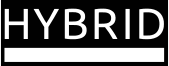
\includegraphics[width=3.5in]{logo}

\vspace{1in}

\today

\vspace{0.5in}

AGREEMENT betweren HYBRID Ink, Ltd (``Publisher'') and \WorkAuthor (``Author''). The parties to this Agreement wish to publish the \WorkType\ ``\WorkTitle'' (``Work'').

\section{Rights}

\paragraph{Author's rights}

The Author retains all rights to the Work not granted to the Publisher below.

\paragraph{Publisher's rights}

The Publisher requests first North American English language print and electronic publication rights to the Work, exclusive for one year. The Publisher does not request rights beyond the first. The Publisher does not request audiobook or film rights.

Here is what this means:

\begin{itemize}
    \item First rights means that the Publisher will be the first ones to publish the work.
    \item North American rights means that the publisher will retain these rights only in The United States and Outlying islands, Mexico, and Canada.
    \item English language rights mean that the publisher only requests the right to publish the Work in English.
    \item Print and electronic rights mean that the publisher requests the rights to publish a print book and an ebook via common services such as Amazon and Barnes \& Nobel for a variety of devices, such as the Kindle and Nook. The Publisher also requests the right to sell the ebook independent of services such as a file download.
    \item Exclusive for one year means that the Publisher requests exclusive rights to publication for one year, after which the publication rights will revert to non-exclusive, allowing the Author to seek subsequent publication elsewhere.
    \item No rights beyond the first, exclusive means that the Publisher is not requesting any further rights for future publication.
\end{itemize}

\section{Indemnifications}

The Author attests that the Work is theirs and, to the best of their knowledge:

\begin{itemize}
    \item Will not infringe on the personal rights of a third party, and
    \item Will not give rise to claims in defamation, privacy, infringement of copyright or trademark, etc.
\end{itemize}

\section{Duties}

\paragraph{Author duties}

The Author shall:

\begin{itemize}
    \item Deliver a complete manuscript for the book,
    \item Work with the Publisher and any representatives on edits, and
    \item Promote and market their own work post-publication.
\end{itemize}

\paragraph{Publisher duties}

The Publisher shall:

\begin{itemize}
    \item Edit the work for content,
    \item Edit the work for spelling and punctuation,
    \item Edit the work for presentation,
    \item Obtain a copyright on the Work if one has not already been obtained,
    \item Procure cover and internal art not otherwise provided by the Author,
    \item Layout and design print and ebooks,
    \item Publish the work, and
    \item Promote and market the work on various channels at their discretion.
\end{itemize}

\section{Advances and Royalties}

\paragraph{Advance}

There will be no advance against future royalties.

\paragraph{Royalties}

The Publisher agrees to pay royalties on net sales according to the following:

\begin{center}
\begin{tabular}{r c}
    \textbf{Edition} & \textbf{Royalties} \\ \hline
    Trade Paperback & \PrintRoyalties \\
    E-book & \DigitalRoyalties \\
    \hline
\end{tabular}
\end{center}

\paragraph{Payment Schedule}

The Publisher will pay the Author quarterly by way of \PaymentMechanism

\section{Publication}

\paragraph{Publication date}

Publication of the Work will not take place after \PublicationDate

\paragraph{Reasonable delay}

Publication may be reasonably delayed due to unforeseeable circumstances through no fault of the Publisher such as, but not limited to, criminal action, labor disputes, etc.

\paragraph{Sunset}

If the publication date is not met by \PublicationDate, this contract will sunset and all rights revert back to the Author.

\end{document}
